\section{Analyse der Struktur}
In diesem Kapitel werden verschiedene dimensionierende Lastfälle vereinfacht berechnet.

\subsection{Allgemeines}

\paragraph{Allgemeine Idealisierung}
SB = Vollidealisiertes Profil -> Rechteck\\
Chassis wird als zwei Längsträger idealisiert, für das Dach werden Profile angenommen. Masse des Profiles angeben inkl. Querschnittsfläche.

\subparagraph{Biegesteifigkeit}
SB ist ein Biegebalken
Widerstandsmoment nicht möglich da unterschiedlicher E-Module -> Biegesteifigkeit $EI$: Gewichtung der Biegesteifigkeiten mit E-Modul
\begin{equation}
  \label{eq:1}
  \begin{split}
    \overline{EI}_y &= \sum A_i \cdot y_i^2 \cdot E_i\\
    \overline{EI}_z &= \sum A_i \cdot z_i^2 \cdot E_i
  \end{split}
\end{equation}
Spannungen:

\begin{equation}
  \label{eq:2}
  \begin{split}
    \sigma &= \frac{M_{b,y}}{\overline{EI}_y}\cdot E_i \cdot y_i\\
    \sigma &= \frac{M_{b,z}}{\overline{EI}_z}\cdot E_i \cdot z_i
  \end{split}
\end{equation}

Schubfluss??? Verhält der? Idealisierung?

\paragraph{Gewichtsverteilung}
Max. Gewicht gemäss Pflichtenheft: 3000kg\\
Angenommene Gewichtsverteilung mit Gewichts-Excel.\\
Vereinfacht angenommen, dass die Deichsel keine Masse hat.
% \begin{center}
%   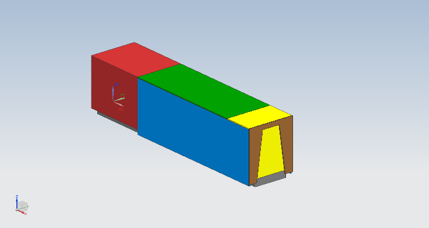
\includegraphics[width=0.5\textwidth]{04_Figures/A.png}
%   \captionof{figure}{Modus A}
%   \label{Modus A}
% \end{center}

\subsection{1.1 Vertikale Beschleunigung}
\paragraph{Idealisierung}
Biegebalken\\
Lagerung:\\
% \begin{center}
%   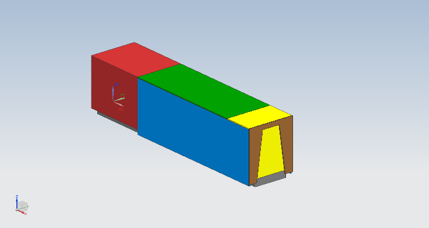
\includegraphics[width=0.5\textwidth]{04_Figures/A.png}
%   \captionof{figure}{Modus A}
%   \label{Modus A}
% \end{center}

\paragraph{Querkraft- und Biegemomentenverlauf}
Querkraftverlauf u. Biegemomentenverlauf durch Integration.\\

\paragraph{Spannungen und Kräfte}
Steifigkeit mit der Formel \ref{eq:1} Spannugen mit der Formel \ref{eq:2}\\
$M_b$,max: Kräfte: 69kN und 420kN

Schubfluss:
Falls SB offen: Schubfluss muss an den Wänden der Küche und Bad abgetragen werden.


\subsection{1.2 Longitudinale Beschleunigung}
\paragraph{Idealisierung}
1.3 wird nicht genommen, da 1.2 grösser ist\\
Starres Chassis: Art und weise der Verzögerung ist egal (Deichsel oder Räder). Berechnung: Druckbelastung wenn alles über die Deichsel verzögert wird: 10MPa...
Trägheitskräfte des Aufbaus wird über die Wände (Feld A und B) aufs Chassis übertragen.
Annahme: Masse ist über die Höhe des SB gleichmässig verteilt. Konservative Annahme das CoG eher tiefer liegt.
Gleichmässge Aufteilung der Masse des mittleren Teiles auf die Felder A und B.

\paragraph{Kräfte und Spannungen}
Feld A, Feld B

\subsection{1.4 Laterale Beschleunigung}
Biegebalken wie bei 1.1 und trägheit des Aufbaus über die Stützen
\paragraph{Biegebalken}
Trägheitskräfte greiffen im Flächenschwerpunk an -> keine Torsion. Gute Annahme.
Lagerung:
Querkraft- und Biegemomentenverlauf:
Normalspannungen:
Schubfluss???

\paragraph{Träger}
1/4 der Masse, Normalverteilt, Querkraft- und Biegemomentenverlauf
Spannungen:

\subsection{1.5 Rotatorische Beschleunigung}












% \section{Komponenten und Verbindungen}
% In diesem Kapitel wird beschrieben, wie der Solar Butterfly aufgebaut ist. Es werden verschiedene Komponenten eingeführt und analysiert wie diese Komponenten miteinander Verbunden sind und welche Kräfte die Verbindungen übertragen müssen.\\
% Weiter wird beschrieben, wie der SB vereinfacht betrachtet wird (Biegebalken) in zwei Moden. (A und C)
%
% \subsection{Komponenten}
% bla bla
%
% \paragraph{Hauptkörper}
% Ganzer Körper als einen Kasten betrachten
% \begin{description}
%   \item \textbf{Chassis}\\
%   Idealisierung: Beam
%   \item \textbf{Boden}\\
%   Auslegung: Biegebalken
%   Idealisierung: Schalenkörper\\
%   \item \textbf{Stützen A und B}\\
%   Auslegung: Schubwand mit Türe\\
%   Profile nehmen Kräfte auf, geben diese Jedoch an die Schubwand weiter\\
%   \item \textbf{Dach}\\
%   Panelen: Schubfläche\\
%   Dach an sich: Biegebalken (Durch eigengewicht)
%   Im Modus \emph{C} Kräfte auf nehmen durch Verriegelung der Seitenwände
% \end{description}
%
% \paragraph{Seitenmodul}
% \begin{description}
%   \item \textbf{Boden}\\
%   Biegebalken und Schubfläche
%   \item \textbf{Seitenwand}\\
%   Modus A: Schubwand\\
%   Modus C: Keine
%   \item \textbf{Ausfahrmechanismus (Scharniere)}\\
%   Wand: Schubwand
%   \item \textbf{}\\
%   \item \textbf{}\\
% \end{description}
